\section{E field using cathode-anode piercing tracks}\label{sec:CAMethod}
\begin{figure}[b]
\centering
\begin{minipage}{0.45\textwidth}
\centering
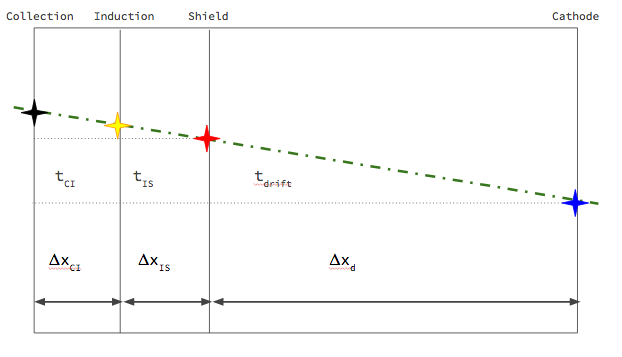
\includegraphics[width=3in]{images/TPCCrossSectionView.png}
\caption{Pictorial representation of the YX view of the TPC. The distance within the anode planes and between the shield plane and the cathode is purposely out of proportion to illustrate the time difference between hits on collection and induciton. A ACP track is shown as an example.}
\label{fig:Scheme}
\end{minipage}\hfill
\begin{minipage}{0.45\textwidth}
\centering
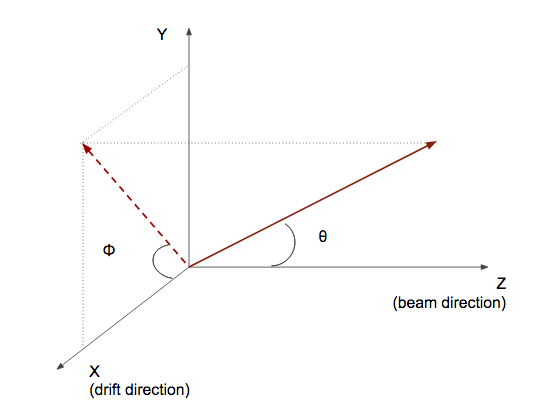
\includegraphics[width=3in]{images/AngleDef.png}
\caption{Angle definition in the context of LArIAT coordinates system.}
\label{fig:AngleDef}
\end{minipage}
\end{figure}

In this section, we propose a method to measure the drift time (and consequently drift velocity and electric field) using TPC data.
The basic idea is simple:
\begin{itemize}
\item[0.] select events with only 1 reconstruced track 
\item[1.] select tracks that cross both anode and cathode,
\item[2.] identify the first and last hit of the track,
\item[3.] measure the time difference between these two hits ($\Delta t$),
\item[4.] derive the drift time from this time difference.
\end{itemize}
We use cosmic data (see section \ref{sec:SampleSelectionCA}) and work under the following assumptions: 
\begin{itemize}
\item [A1.] the selected tracks are muons in the MIP region
\item [A2.] the time it takes for a muon to cross the chamber ($\sim$ns) is irrelevant compared to the charge drift time ($\sim$ hundreds of $\mu$s).
\end{itemize}

We select events with only one recontructed track to assure the track considered in the analysis is associated with the trigger.
We select anode-cahode piercing tracks (ACP tracks in what follows) because their hits span the full drift lenght of the TPC, see figure \ref{fig:Scheme}. It is important to define where the first and last hit of the tracks are located. The definition of the last hit is easy: it is the hit closest to the cathode. The definition of the first hit is a bit more complicated. A track that crosses the anode planes will deposit charge in the small drift volumes (CI and IS). We calculated the dift time in IS and CI in table \ref{tab:Efields}: $\Delta t_{IS} = 2.31  \mu s$  and $\Delta t_{CI} = 2.11 \mu s $ respectvely. This is to say that the position of the first hit  matters when calculating the drift time at the microsecond precision.
Single hits on the collection plan will not form a 3D object. This means that we can safely exclude that the reconstruction of ACP tracks starts at the cathode plane (black point in figure \ref{fig:Scheme}). Understanding if the first hit of a track in on the induction or on the shield plan is more complicated. For now, we'll take an uncertainty hit of 2.3 $\mu$s.


One of the main features of this method is that it doesn't rely on the measurement of the trigger time. Since $\Delta t$ is the time difference between the first and last hit of a track and we assume the charge started drifting at the same time for both hits (assumption A2), the measurement of the absolute beginning of drift time $t_0$ is unnecessary. 


\subsection{Andode-Cathode Piercing Tracks Sample Selection}\label{sec:SampleSelectionCA}

The data samples used for this measurement span RunI and RunII. The data are divided into three independent subsamples: RunI positive polarity data, RunII positive polarity data and RunII negative polarity data. Since we're interested in cosmics, this organization is arbirtary and only dictated by the subsamples availability.
More details are shown in table \ref{tab:samples}, while the samweb definitions are defined at the end of \href{https://redmine.fnal.gov/redmine/projects/lardbt/wiki/Recommended_SAM_Datasets}{this wiki page}.

\begin{center}
\begin{table}[htb]
  \begin{center}
    %\resizebox{0.45\textwidth}{!}{%
    \begin{tabular}{c|c|c|c}
      \multicolumn{4}{c}{\textbf{Summary of Samples}} \\
      \hline \hline
       Run Period & LArIATsoft Version & Data Polarity  & SamWeb definition\\
       \hline
       Run-I & \verb!v06_34_01! & Positive &  \verb!Lovely1_Pos_RunI_elenag_v04!\\
       \hline
       Run-II & \verb!v06_34_01! & Positive  & \verb!Lovely1_Pos_RunII_elenag_v04! \\
       \hline
       Run-II & \verb!v06_34_01! & Negative  & \verb!Lovely1_Neg_RunII_elenag_v04! \\
       \hline
       \end{tabular}%}
    \caption{Summary of the data samples used for the Anode-Cathode Piercing tracks study. }
    \label{tab:samples}
    \end{center}
\end{table}
\end{center}

For each sample, the same event selection is used: we outline it in what follows.
\begin{itemize}
\item \textbf{Time Stamp Filter}

A filter is used to select events which occured outside the beam window. This is because the beam is mainly focused in the Z direction, so ACP tracks are unlikely to occur during the beam spill. Cosmics events typically occur 5.5 seconds past the beam spill, and therefore the events are filtered using the following LArIATsoft settings

\begin{verbatim}
tfilt:      @local::lariat_timestampfilter

# ====================================================================
# Specify range of events to select.  For Run I/II:
#   - pedestal events:  ~ 0.  - 1.2 sec
#   - beam events:      ~ 1.2 - 5.5 sec
#   - cosmic events:    ~ > 5.5 sec
#   (default selects ALL events)
physics.filters.tfilt.T1:                       5.5
physics.filters.tfilt.T2:                       100.
physics.filters.tfilt.RequireRawDigits:         true

\end{verbatim}


\item \textbf{LArTPC Reconstruction}

Events are then reconstructed inside the TPC. Since we only want ACP tracks, we select tracks that satisfy the following requirements

\begin{itemize}
\item vertical position (Y) of first and last hits within $\pm$ 18 cm from TPC center (avoid Top-Bottom tracks) 
\item horizonatl position (Z) of first and last hits within 2 and 86 cm from TPC front face (avoid throughoing tracks) 
\item longest track with track lenght greater than 48 cm
\item angle from the drift direction (phi in figure \ref{fig:AngleDef}) smaller than 50 deg 
\item angle from the beam direction (theta in figure \ref{fig:AngleDef}) grater than 60 deg
\end{itemize}




\end{itemize}

Tracks passing all these selection requirements are used for the $\Delta t$ calculation.


\subsection{Hit timing information}\label{sec:HitTime}
For each track passing our selection, we loop through the associated hits in order to retrieve the timing information. Hits on the collection and hits on the induction are treated separately. Three types of timing information are provided per each hit: tStart, tPeak and tEnd. The quantities tStart and tEnd are used to identify a region of interest on the signal wave form in each wire. This ROI is represent the time boundary where a fit for the signal peak is performed. The variable tPeak stores the fitted value for the time of the hit. For this analysis, we use \verb!gaushitfinder! and the variable tPeak as a measure of the hit time.


Figure \ref{fig:RunIPosACP} represents the difference in time between the last and first hit of the selected ACP tracks for RunI Positive Polarity sample. The red histogram represents $\Delta$t calculated with hits on induction plan, while the blue histogram histogram represents $\Delta$t calculated with hits on the collection plan.
Figure \ref{fig:RunIIPosACP} and \ref{fig:RunIINegACP} are analougus to figure \ref{fig:RunIPosACP} for RunII Positive and Negative polarity respectively.

\begin{figure}[b]
\centering
\begin{minipage}{0.45\textwidth}
\centering
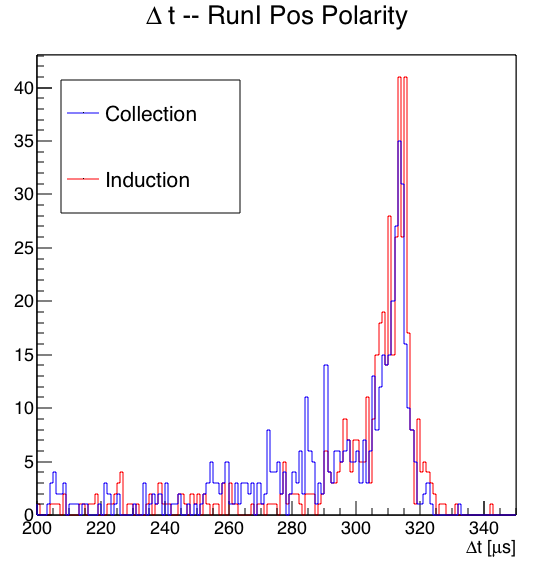
\includegraphics[width=3in]{images/ACPRunIPos.png}
\caption{$\Delta$t for Run I positive polarity data ACP selected tracks. The blue line represents hits on the collection plan, red induction.}
\label{fig:RunIPosACP}
\end{minipage}\hfill
\begin{minipage}{0.45\textwidth}
\centering
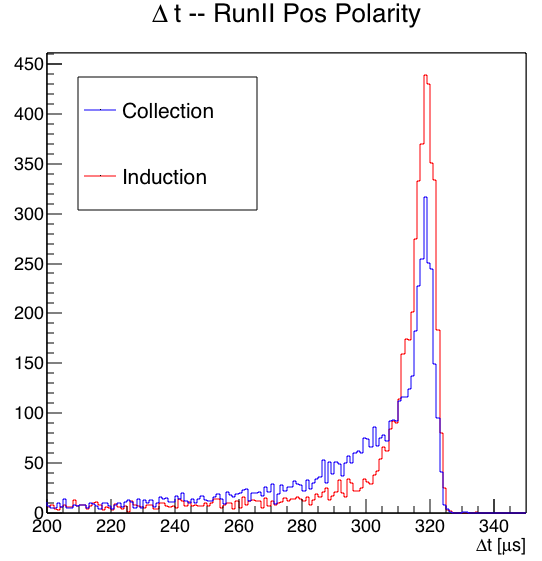
\includegraphics[width=3in]{images/ACPRunIIPos.png}
\caption{$\Delta$t for Run II positive polarity data ACP selected tracks.  The blue line represents hits on the collection plan, red induction.}
\label{fig:RunIIPosACP}
\end{minipage}\hfill
\begin{minipage}{0.45\textwidth}
\centering
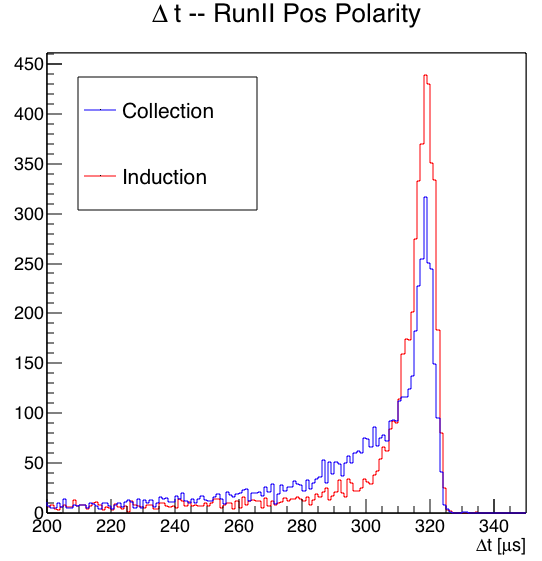
\includegraphics[width=3in]{images/ACPRunIIPos.png}
\caption{$\Delta$t for Run II negative polarity data ACP selected tracks.  The blue line represents hits on the collection plan, red induction.}
\label{fig:RunIINegACP}
\end{minipage}
\end{figure}

We fit with a gaussian the peak in figures  \ref{fig:RunIPosACP}, \ref{fig:RunIIPosACP} and \ref{fig:RunIINegACP}. An example of the fit is shown in figures \ref{fig:CollFit} and \ref{fig:IndFit}. We use the mean as our estimate of $\Delta t$ and the sigma as it error. The $\Delta t$ value for each distribution is shown in table \ref{tab:deltaTACP}.
\begin{figure}[b]
\centering
\begin{minipage}{0.45\textwidth}
\centering
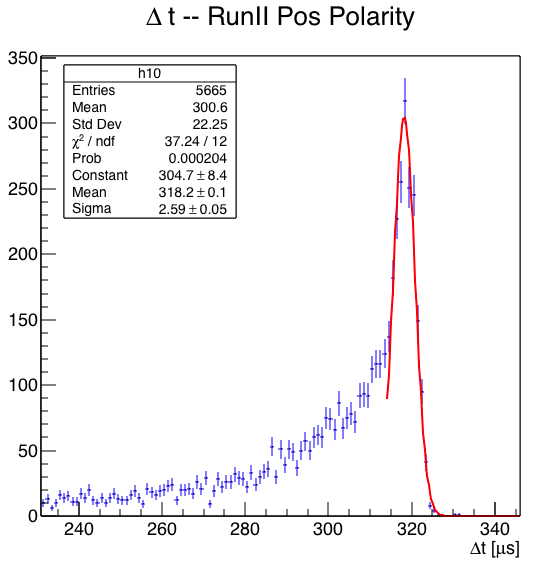
\includegraphics[width=3in]{images/CollectionFitRunIIPos.png}
\caption{Collection plan $\Delta$t fit  for Run I positive polarity data ACP selected tracks. }
\label{fig:CollFit}
\end{minipage}\hfill
\begin{minipage}{0.45\textwidth}
\centering
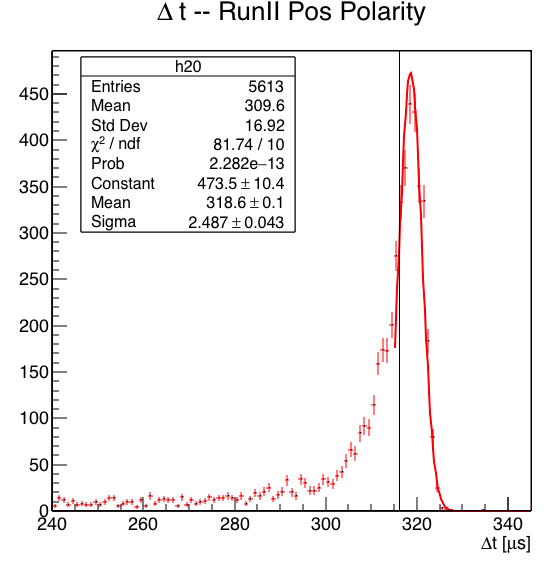
\includegraphics[width=3in]{images/InductionFitRunIIPos.png}
\caption{Collection plan $\Delta$t fit  for Run I positive polarity data ACP selected tracks. }
\label{fig:IndFit}
\end{minipage}
\end{figure}

\begin{center}
\begin{table}[htb]
  \begin{center}
    %\resizebox{0.45\textwidth}{!}{%
    \begin{tabular}{|c|c|}
      \multicolumn{2}{c}{\textbf{Delta t for ACP tracks}} \\
      \hline \hline
       Data Period  & $\Delta t$ [$\mu s$] \\
       \hline
       RunI Positive Polarity Induction & 313.7 $\pm$ 2.1 \\
       \hline
       RunI Positive Polarity Collection & 313.2 $\pm$ 2.6 \\
       \hline
       RunII Positive Polarity Induction &  318.6 $\pm$ 2.5\\
       \hline
       RunII Positive Polarity Collection & 318.2 $\pm$ 2.6 \\
       \hline
       RunII Negative Polarity Induction &  $\pm$ \\
       \hline
       RunII Negative Polarity Collection & $\pm$ \\
       \hline
       \end{tabular}
    \caption{$\Delta t$ for the different data samples used for the Anode-Cathode Piercing tracks study. }
    \label{tab:deltaTACP}
    \end{center}
\end{table}
\end{center}


For the RunII Positive polarity data, we scan plot the position of the peak as a function of the angle theta and phi. Figures \ref{fig:RunIPosACPTheta} and \ref{fig:RunIIPosACPPhi} show the trends.
\begin{figure}[b]
\centering
\begin{minipage}{0.45\textwidth}
\centering
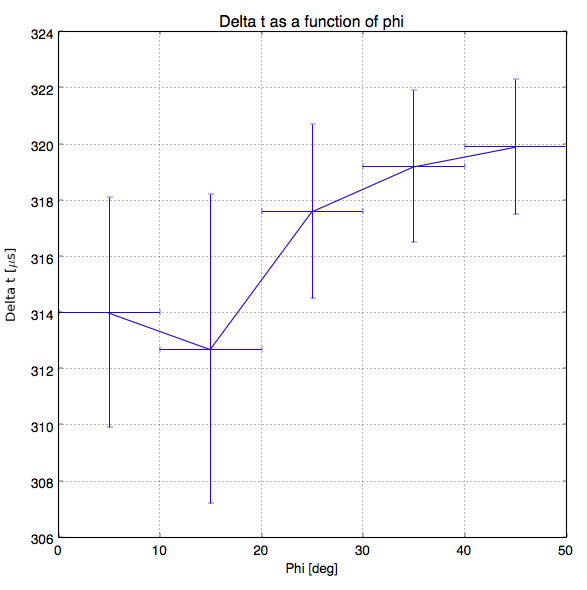
\includegraphics[width=3in]{images/CollectionFitRunIIPosPhi.png}
\caption{$\Delta$t for Run II positive polarity data ACP selected tracks as a function of Phi. }
\label{fig:RunIPosACPTheta}
\end{minipage}\hfill
\begin{minipage}{0.45\textwidth}
\centering
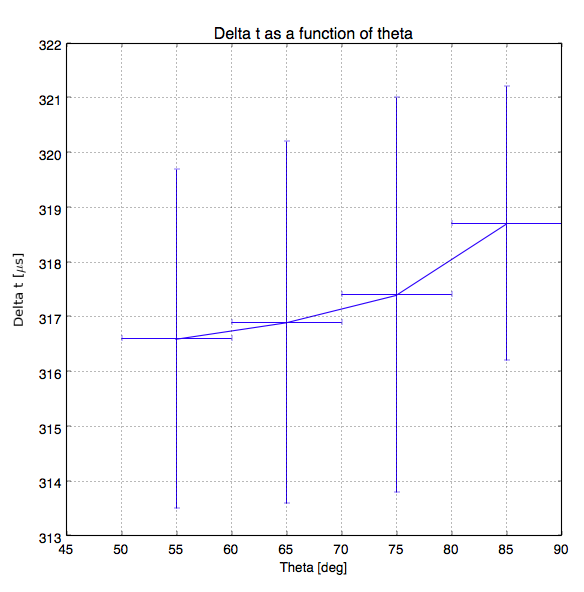
\includegraphics[width=3in]{images/CollectionFitRunIIPosTheta.png}
\caption{$\Delta$t for Run II positive polarity data ACP selected tracks as a function of Theta.}
\label{fig:RunIIPosACPPhi}
\end{minipage}
\end{figure}
\clearpage
\newpage
